\chapter{Connectedness and Compactness}

\section{Connectedness}
\subsection{Definition~2.1}

The equivalence of the two conditions will be shows in \nameref{exercise 2.1} (page~\pageref{exercise 2.1}).

\subsection{Theorem~2.2}



\subsubsection{Path Connectedness}

Suppose that each~$X_α$ is path connected.

Let~$∼$ be the equivalence relation on~$X$ given by
\[
	x ∼ y
	\iff
	\text{there exists a path between~$x$ and~$y$ in~$X$} \,.
\]
We have already seen underneath Definition~2.2 that~$∼$ is indeed an equivalence relation on~$X$.
It follows for every index~$α$ and every point~$y$ in~$X_α$ from the path connectedness of~$X_α$ that~$y ∼ x$.
(We use here the universal property of the subspace topology, which ensures that every path in~$X_α$ is also a path in~$X$.)
This tells us that every point of~$X$ is equivalent to~$x$ with respect to~$∼$, because~$X$ is covered by the sets~$X_α$.
By the transitivity of~$∼$, all points of~$X$ are equivalent with respect to~$∼$.

Therefore,~$X$ is path connected.



\subsubsection{Connected}

Suppose that each~$X_α$ is connected.

Let~$f$ be a continuous map from~$X$ to~$\{ 0, 1 \}$, where~$\{ 0, 1\}$ is endowed with the discrete topology.
For every index~$α$, the restriction~$\restrict{f}{X_α}$ is a continuos map from~$X_α$ to~$Y$ (because it is the composite of~$f$ and the inclusion map from~$X_α$ to~$X$, which is continuous).
It follows for every index~$α$ that~$\restrict{f}{X_α}$ is constant because~$X_α$ is connected;
let~$c_α ∈ \{ 0, 1 \}$ be the constant value of~$\restrict{f}{X_α}$ (we use here that~$X_α$ is nonempty since it contains the point~$x$).
We have~$f x = c_α$ for every index~$α$, whence all~$c_α$ are equal.
This tells us that~$f$ is constant on~$⋃_{α ∈ A} X_α = X$.

This shows that~$X$ is connected.

\subsection{Example~2.1}

Let~$X$ be a subspace of~$ℚ$ that consists of at least two distinct elements$~x$ and~$y$.
We may assume that~$x < y$.
There exists an irrational number~$a$ with~$x < a < y$.
The sets
\[
	U = \{ z ∈ X \suchthat z < a \} \,,
	\quad
	V = \{ z ∈ X \suchthat z > a \}
\]
are disjoint, nonempty, and open in~$X$, with~$X = U ∪ V$.
The existence of these sets shows that~$X$ is not connected.

This shows that~$ℚ$ is indeed totally disconnected.

\subsection{The Functor~\texorpdfstring{$\fgroup_0$}{π\_0}~(2.1.2)}

Instead of saying that~\enquote{$f A$ is connected} we need to say that~\enquote{$f A$ is path connected}.

\subsection{Constructions and Connectedness~(2.1.3)}

We have seen that~$ℝ$ is connected, but its subspace~$ℚ$ is note.
Therefore, connectedness is not inherited by subspaces.

That the disjoint union of two connected spaces won’t be connected is only true if both spaces are also assumed to be nonempty.

\subsection{Theorem~2.9}

\begin{proposition}
	\label{product with singleton is homeomorphic to original space}
	Let~$X$ be a topological space and let~$Y ≔ \{ y \}$ be one-point topological space
	Then~$X × Y ≅ X$.
\end{proposition}

\begin{proof}
	The map
	\[
		φ \colon X \to X × Y \,, \quad x \mapsto (x, y)
	\]
	is continuous in both coordinates by the universal property of the product topology.
	The map
	\[
		ψ \colon X \to X × Y \,, \quad (x, y) \mapsto x
	\]
	is the projection onto the first coordinate, and thus also continuous.
	The two continuous maps~$φ$ and~$ψ$ are mutually inverse, whence~$φ$ is a homeomorphism with inverse given by~$ψ$.
\end{proof}

Let~$X ≔ \prod_{α ∈ A} X_α$.
Let~$f$ be a continuous map from~$X$ to~$\{ 0, 1 \}$, where~$\{ 0, 1 \}$ is endowed with the discrete topology.
We show in the following that~$f$ is constant.

For every point~$x = (x_α)_α$ in~$X$ and every index~$β$ we can consider the set
\[
	X_{x, β}
	≔
	\{ (y_α)_α ∈ X \suchthat \text{$y_α = x_α$ whenever~$α ≠ β$}  \}
	=
	∏_{α ∈ A}
	\begin{cases*}
		X_β       & if~$α = β$, \\
		\{ x_α \} & otherwise.
	\end{cases*}
\]
Under the associativity homeomorphism~$X ≅ X_β × ∏_{α ≠ β} X_α$, the set~$X_{x, β}$ corresponds to~$X_β × \{ (x_α)_{α ≠ β} \}$.
According to~\cref{product with singleton is homeomorphic to original space}, and because the product topology and subspace topology are compatible, the subspace~$X_{x, β}$ of~$X$ is homeomorphic to~$X_β$ and thus connected.
It follows that~$f$ is constant on~$X_{x, β}$.

This shows that~$f x = f y$ whenever two elements~$x$ and~$y$ of~$X$ differ only in one coordinate.
It follows by induction that~$f x = f y$ whenever~$x$ and~$y$ differ only in finitely many coordinates.

Let now~$x = (x_α)_α$ be some point in~$X$.
We will show that~$f x = f y$ for every~$y ∈ X$.
To this end we may assume that~$f x = 0$ (because otherwise we can replace the map~$f$ by the map~$f'$ with~$f' y = 1 - f y$).
The preimage~$V ≔ f^{-1} \{ 0 \}$ is an open subset of~$X$ that contains~$x$.
There hence exists an open subset~$U$ of~$X$ of the form~$U = ∏_{α ∈ A} U_α$, with~$U_α$ open in~$X_α$ for every~$α$ and~$U_α = X_α$ for all but finitely many~$α$, such that~$x ∈ U$ and~$U ⊆ V$.

Let~$A' ≔ \{ α ∈ A \suchthat U_α = X_α \}$.
This set is cofinite in~$A$, i.e., all but finitely many elements of~$A$ are contained in~$A'$.
We note that we can change all coordinates~$x_α$ for~$α ∈ A'$ without leaving the set~$U$, and thus without leaving the preimage~$f^{-1} \{ 0 \}$.

Let~$y = (y_α)_α$ be another point in~$X$.
To show that~$f y = 0$, we consider the auxiliary point~$z = (z_α)_α$ in~$X$ given by the coordinates
\[
	z_α
	=
	\begin{cases*}
		y_α & if~$α ∈ A'$, \\
		x_α & otherwise.
	\end{cases*}
\]
The point~$z$ is again contained in the set~$U$, and thus contained in~$f^{-1} \{ 0 \}$, so that~$f z = 0$.
But~$y$ and~$z$ differ only in finitely many entries, whence furthermore~$f y = f z = 0$.

\subsection{Theorem~2.10}

We will prove this theorem in \nameref{exercise 2.6}.

\subsection{Theorem~2.11}

We give a proof of this theorem in \nameref{exercise 2.7}.

\subsection{Example~2.2}

We denote the given space by
\[
	X = \{ 0 \} × [-1, 1] ∪ \{ (x, \sin(1/x)) \suchthat x > 0 \} \,.
\]



\subsubsection{$X$ is connected}

The space~$X$ consists of two components:
the line~$L ≔ \{ 0 \} × [-1, 1]$ and the curve~$C = \{ (x, \sin(1 / x)) \suchthat x > 0 \}$.
Both subspaces of~$X$ are connected since they are the images of connected spaces under continuous maps, namely
\[
	[0, 1] \to L \,, \quad t \mapsto (0, 2t - 1)
\]
and
\[
	(0, ∞) \to C \,, \quad x \mapsto (x, \sin(1 / x)) \,.
\]
(These maps are in fact homeomorphisms).

Let~$f \colon X \to \{ 0, 1 \}$ be a continuous map, where~$\{ 0, 1 \}$ is endowed with the discrete topology.
The map~$f$ is constant on both~$L$ and~$C$.
Let~$x ≔ (0, 0)$ and let~$c ≔ f x$.
The preimage~$f^{-1} \{ c \}$ is an open subset of~$X$ containing~$x$.
There hence exists some~$ε > 0$ for which the set~$\ball(x, ε) ∩ X$ is contained in~$f^{-1} \{ c \}$.
The set~$\ball(x, ε) ∩ X$ contains the point~$x$ of the line~$L$ but also points of the curve~$C$.
It follows that~$f$ is constant with value~$c$, since~$f$ is constant on both~$L$ and~$C$.

This shows that the space~$X$ is connected.



\subsubsection{$X$ is not path connected}

Let $x_0 ≔ (1/(\pi/2), 1) ∈ C$, and suppose that there exists a path~$γ \colon [0, 1] \to X$ from~$x_0$ to~$x = (0, 0)$.
Let~$π$ be the projection from~$ℝ^2$ to~$ℝ$ restricted to a continuous map from~$X$ to~$[0, ∞)$.
The composite~$π γ$ is a path in~$[0, ∞)$ from~$1/(\pi/2)$ to~$0$.
It follows from repeated usage of the intermediate value theorem that there exist an increasing sequence
\[
	\frac{1}{\pi/2} = t_0 < t_1 < t_2 < t_3 < \dotsb ≤ 1
\]
with
\[
	π γ t_n = \frac{1}{(n + \frac{1}{2}) \pi}
\]
for every~$n ≥ 0$.
It follows that
\[
	γ t_n = ( t_n, (-1)^n )
\]
for every~$n ≥ 0$.
The sequence~$(t_n)_n$ is strictly increasing and bonded from above, and thus convergent.
It follows that the sequence~$(γ t_n)_n$ again converges, because~$γ$ is continuous.
By projecting onto the second coordinate, we finally find that the sequence~$( (-1)^n )_n$ converges.
What nonsense!

\subsection{Locally Connected Spaces Have Open Connected Components}

The book never defined what a neighbourhood is (only the concept of an open neighbourhood is defined, in Definition~0.2).
Let’s fix this.

\begin{definition}
	Let~$X$ be a topological space and let~$x$ be a point in~$X$.
	A subset~$N$ on~$X$ is a \defemph{neighbourhood} of~$x$ if there exists an open subset~$U$ of~$X$ with~$x ∈ U$ and~$U ⊆ N$.
\end{definition}

Open sets can be characterized in terms of neighbourhoods:

\begin{proposition}
	Let~$X$ be a topological space.
	A subset~$U$ of~$X$ is open if and only if it is a neighbourhood of each of its points.
\end{proposition}

\begin{proof}
	If~$U$ is open, then there exists for every point~$x$ in~$X$ an open subset~$V$ of~$X$ with~$x ∈ V$ and~$V ⊆ U$, namely~$V = U$.
	In other words, the set~$U$ is a neighbourhood for each of its points.

	Suppose conversely that~$U$ is a neighbourhood for each of its points.
	Then there exists for every point~$x$ in~$U$ an open subset~$V_x$ of~$X$ with~$x ∈ V_x$ and~$V_x ⊆ U$.
	It follows that~$U = ⋃_{x ∈ X} V_x$ is a union of open subsets of~$X$, and therefore itself open in~$X$.
\end{proof}

Let~$X$ be a locally connected topological space and let~$C$ be a connected component of~$X$.

Let~$x$ be a point in~$C$.
The point~$x$ admits by assumption a connected neighbourhood~$N$.
The connected component~$C$ is a superset of~$N$ because~$N$ is a connected subspace of~$X$ containing~$x$.
This shows that~$C$ contains a neighbourhood of~$x$, and is therefore itself a neighbourhood of~$x$.

We have shown that the connected component~$C$ is a neighbourhood for each of its points.
In other words,~$C$ is open.

\subsection{Theorem~2.12}

Let~$X$ be a topological space.
We denote the path components of~$X$ by~$P_α$ with~$α ∈ A$, and the connected components by~$C_β$ with~$β ∈ B$.
We have the set-theoretic decompositions~$X = ∐_{α ∈ A} P_α$ and~$X = ∐_{β ∈ B} C_β$.

Every path component is connected and therefore contained in a connected component.
It follows that the decomposition~$X = ∐_{α ∈ A} P_α$ is finer than the decomposition~$X = ∐_{β ∈ B} C_β$, i.e., there exists a decomposition~$A = ∐_{β ∈ B} A_β$ with~$C_β = ∐_{α ∈ A_β} P_α$ for every~$β ∈ B$.

Suppose now that~$X$ is locally path connected.
Every path components~$P_α$ is then open in~$X$.
It follows that~$C_β = ∐_{α ∈ A_β} P_α$ is a decomposition into pairwise disjoint, nonempty, open subsets of~$X$, and therefore also open subsets of~$C_β$.
But~$C$ is connected, so this decomposition must be trivial:
The set~$A_β$ consists of only a single element~$α(β)$, and we have~$C_β = P_{α(β)}$.

The decomposition~$X = ∐_{α ∈ A} P_α$ is therefore not \emph{strictly} finer than the decomposition~$X = ∐_{β ∈ B} C_β$.
Therefore, both decompositions agree, whence the connected components and path components agree.

\subsection{Example~2.4}



\subsubsection{$X$ is path connected}

The horizontal line~$L ≔ [0, 1] × \{ 0 \}$ is homeomorphic to the interval~$[0, 1]$ and therefore path-connected.
For every~$x ∈ C$, the tooth~$T_x ≔ \{ x \} × [0, 1]$ of the comb~$X$ is also homeomorphic to~$[0, 1]$ and therefore path-connected.
The line~$L$ and tooth~$T_x$ intersect in the point~$(x, 0)$ of~$X$, and are therefore both contained in the same path component of~$X$.

It follows that the path component of~$X$ that contains~$L$ also contains every tooth~$T_x$ with~$x ∈ C$, and contains therefore all of~$X$.
In other words, the space~$X$ is path connected.



\subsubsection{$X$ is not locally path connected}

We start by making an important observation.

Let~$π \colon X \to [0, 1]$ be th projection onto the first coordinate
Let~$x$ and~$x'$ be two points in~$C$ and let~$γ \colon [0, 1] \to X$ be a path from~$y ≔ (x, 1)$ to~$y' ≔ (x', 1)$.
There exists a number~$x''$ between~$x$ and~$x'$ that is not contained in~$C$.
By the intermediate value theorem, there exists some~$t ∈ [0, 1]$ with~$π γ t = x''$.
The original point~$γ t$ in~$X$ needs to be given by~$γ t = (x'', 0)$ since this is the only preimage of~$x''$ under~$π$.

This tells us that any path between two tips of the comb needs to pass through the horizontal line~$L$ at some point.
See also \cref{path must pass through the horizontal line}.
\begin{figure}
	\centering
	\begin{tikzpicture}
		% horizontal line
		\draw (-2, 0) node[left] {$\cdots$} -- (5, 0) node[right] {$\cdots$};
		% vertical lines
		\draw (-1.5, 0) -- (-1.5, 3) ;
		\draw (0, 0) -- (0, 3) node[above] {$(x, 1)$};
		\draw (2, 0) -- (2, 3) node[above] {$(x', 1)$};
		\draw (4.5, 0) -- (4.5, 3);
		% the path
		\draw[very thick, ->] (0, 3) -- (0, 0) -- (2, 0) -- (2, 3);
		% point between the teeths of the comb
		\draw (1, 0.1) -- (1, -0.1) node[below] {$(x'', 0)$};
	\end{tikzpicture}
	\caption{Every paths between tips must pass through the horizontal line.}
	\label{path must pass through the horizontal line}
\end{figure}

Suppose that the space~$X$ were locally path connected.
We consider then the point~$p ≔ (0, 1)$ in the upper-left corner of the comb, and its open neighbourhood
\[
	V ≔ [0, 1] × (1/2, 1]
\]
that consists of the open upper half of the comb.
There exists by assumption a path-connected neighbourhood~$U$ of~$p$ with~$U ⊆ V$.
There exists a radius~$ε > 0$ with~$\ball(p, ε) ∩ X ⊆ U$.
For a sufficiently large integer~$n$ we have~$1/n < ε$.
The two comb tips~$y ≔ (1/(n + 1), 1)$ and~$y' ≔ (1/n, 1)$ are contained in~$\ball(p, ε) ∩ X$, and are therefore contained in~$U$.
There exists a path~$γ$ from~$y$ to~$y'$ in~$U$ because~$U$ is path connected.

We can regard~$γ$ as a path from~$y$ to~$y'$ in~$X$.
We have seen above that the path~$γ$ needs to pass through the horizontal line~$L$ at some point.
But this cannot be, because~$γ$ is completely contained in~$V$ and~$V$ is disjoint to~$L$.

This shows that~$X$ cannot be locally path connected.


\section{Hausdorff Spaces}
\subsection{Constructions with Hausdorff Spaces}



\subsubsection{Topological Property}

\begin{lemma}
	\label{pull back Hausdorff via injective continuous maps}
	Let~$X$ and~$Y$ be two topological spaces.
	Let~$Y$ be a Hausdorff space and suppose that there exists an injective continuous map from~$X$ to~$Y$.
	Then~$X$ is again a Hausdorff space.
\end{lemma}

\begin{proof}
	Let~$f$ be an injective continuous map from~$X$ to~$Y$.

	Let~$x$ and~$x'$ be two distinct points in~$X$.
	The two points~$f x$ and~$f x'$ in~$Y$ are again distinct because~$f$ is injective.
	There exist disjoint open neighbourhoods~$V$ and~$V'$ of~$f x$ and~$f x'$ respectively.
	The preimages~$f^{-1} V$ and~$f^{-1} V'$ are disjoint open neighbourhoods of~$x$ and~$x'$ respectively.
\end{proof}

Let~$X$ and~$Y$ be two homeomorphic topological spaces.
It follows from \cref{pull back Hausdorff via injective continuous maps} that~$X$ is a Hausdorff space if and only if~$Y$ is a Hausdorff space.



\subsubsection{Not a Homotopy Invariant Property}

\begin{lemma}
	\label{all maps into indiscrete are homotopic}
	Let~$X$ be a topological space and let~$Y$ be an indiscrete topological space.
	Every two maps from~$X$ to~$Y$ are homotopic.
	\qed
\end{lemma}

It follows from \cref{all maps into indiscrete are homotopic} that all nonempty indiscrete topological spaces are homotopy equivalent.
The one-point space is a Hausdorff space, whereas the two-point indiscrete topological space is not.



\subsubsection{Subspaces of Hausdorff Spaces}

Let~$X$ be a Hausdorff space and let~$Y$ be a subspace of~$X$.
It follows from \cref{pull back Hausdorff via injective continuous maps} that~$Y$ is again a Hausdorff space.



\subsubsection{Products of Hausdorff Spaces}

Let~$(X_α)_{α ∈ A}$ be a family of topological spaces and suppose that each~$X_α$ is a Hausdorff space.
Let~$x = (x_α)_α$ and~$y = (y_α)_α$ be two distinct elements of~$∏_{α ∈ A} X_α$.
This means that there exist some index~$β$ with~$x_β ≠ y_β$.
The space~$X_β$ is a Hausdorff space, so there exists disjoint open neighbourhoods~$U$ and~$V$ of~$x_β$ and~$y_β$ respectively.
The preimages~$π_β^{-1} U$ and~$π_β^{-1} V$ are disjoint open neighbourhoods of~$x$ and~$y$ respectively.



\subsubsection{Coproducts of Hausdorff Spaces}

Let~$(X_α)_α$ be a family of Hausdorff spaces and let~$x$ and~$y$ be two elements of the coproduct~$X ≔ ∐_{α ∈ A} X_α$.
There exist indices~$α, β ∈ A$ with~$x ∈ X_α$ and~$y ∈ X_β$.
We distinguish between two cases:

\begin{casedistinction}

	\item
		Suppose that~$α ≠ β$.
		Then~$X_α$ and~$X_β$ are disjoint open neighbourhoods of~$x$ and~$y$ in~$X$ respectively.

	\item
		Suppose that~$α = β$.
		Then there exist disjoint open neighbourhoods of~$x$ and~$y$ in~$X_α$.
		These are then also disjoint open neighbourhoods of~$x$ and~$y$ in~$X$.

\end{casedistinction}



\subsubsection{Quotients of Hausdorff Spaces}

Let~$∼$ be the equivalence relation on~$ℝ$ given by
\[
	x ∼ y \iff \text{$x - y$ is rational} \,.
\]
That is, for every point~$x$ in~$ℝ$, its equivalence class is~$x + ℚ$.

Let~$U$ be nonempty saturated open subset of~$ℝ$.
The set~$U$ contains some open interval~$I = (a, b)$ with~$a < b$.
It follows that~$⋃_{x ∈ I} x + ℚ ⊆ U$ because~$U$ is saturated, but~$⋃_{x ∈ I} x + ℚ = ℝ$ since for every real number~$r$ there exists a rational number~$q$ with~$a < r + q < b$.
Therefore,~$U = ℝ$.

This shows that the only saturated open subsets of~$ℝ$ are~$∅$ and~$ℝ$.
This means that the quotient topology on~$ℝ / {∼}$ is indiscrete.
But~$ℝ / {∼}$ is uncountable since~$ℝ$ is uncountable but each equivalence class with respect to~$ℚ$ is only countable.

So while~$ℝ$ is a Hausdorff space, its quotient~$ℝ / {∼}$ is very much not a Hausdorff space.

\subsection{Theorem~2.14}

We show that for every topological space~$X$ the following conditions are equivalent:
\begin{equivalenceslist}

	\item
		\label{space is hausdorff}
		$X$ is a Hausdorff space.

	\item
		\label{diagonal set is closed}
		The diagonal set~$Δ_X = \{ (x, x) \suchthat x ∈ X \}$ is closed in~$X × X$.

	\item
		\label{diagonal map is closed}
		The diagonal map~$Δ \colon X \to X × X$,~$x \mapsto (x, x)$ is closed.

\end{equivalenceslist}

We note that two subsets~$U$ and~$V$ of~$X$ are disjoint if and only if the subset~$U × V$ of~$X × X$ is disjoint to~$Δ_X$.
For the equivalence of~\ref{diagonal set is closed} and~\ref{space is hausdorff} we observe the chain of equivalences
\begingroup
\allowdisplaybreaks
\begin{align*}
	{}&
	\text{$Δ_X$ is closed} \\
	\iff{}&
	\text{$(X × X) ∖ Δ_X$ is open} \\
	\iff{}&
	\left\{
	\begin{tabular}{l}
		for every~$(x, y) ∈ (X × X) ∖ Δ_X$ \\
		there exists~$W ⊆ X × X$ open \\
		with~$(x, y) ∈ W ⊆ (X × X) ∖ Δ_X$
	\end{tabular}
	\right. \\
	\iff{}&
	\left\{
	\begin{tabular}{l}
		for every~$(x, y) ∈ (X × X) ∖ Δ_X$ \\
		there exists~$U, V ⊆ X$ open \\
		with~$(x, y) ∈ U × V ⊆ (X × X) ∖ Δ_X$
	\end{tabular}
	\right. \\
	\iff{}&
	\left\{
	\begin{tabular}{l}
		for all~$x, y ∈ X$ with~$x ≠ y$ \\
		there exists~$U, V ⊆ X$ open \\
		with~$x ∈ U$,~$y ∈ V$ and~$U$ and~$V$ are disjoint
	\end{tabular}
	\right. \\
	\iff{}&
	\text{$X$ is Hausdorff} \,.
\end{align*}
\endgroup

For the equivalence of~\ref{diagonal set is closed} and~\ref{space is hausdorff} we note that the two maps
\[
	φ \colon X \to Δ_X \,, \quad x \mapsto (x, x)
\]
and
\[
	ψ \colon Δ_X \to X \,, \quad (x, x) \mapsto x
\]
are continuous and mutually inverse.
(The continuity of~$φ$ follows from the universal property of the product topology and the universal property of the subspace topology.
The map~$ψ$ is continuous because it is the restriction of the canonical projection maps.)
The maps~$φ$ and~$ψ$ are mutually inverse, whence~$φ$ is a homeomorphism with inverse~$ψ$.

Suppose that~$Δ_X$ is closed in~$X$.
Then for every subset~$C$ of~$Δ_X$, the set~$C$ is closed in~$Δ_X$ if and only if~$C$ is closed in~$X × X$.
It follows for every subset~$C$ of~$X$ that
\begin{align*}
	\SwapAboveDisplaySkip
	{}&
	\text{$C$ is closed in~$X$} \\
	\iff{}&
	\text{$φ C$ is closed in~$Δ_X$} \\
	\iff{}&
	\text{$φ C$ is closed in~$X × X$} \\
	\iff{}&
	\text{$Δ C$ is closed in~$X × X$} \,.
\end{align*}
This means that the map~$Δ$ is closed.

If conversely~$Δ$ is closed, then it follows in particular that~$Δ X$ is closed in~$X × X$.
But~$Δ X = Δ_X$.


\section{Compactness}
\subsection{Theorem~2.15}

Let~$f \colon X \to Y$ be a surjective continuous map and suppose that~$X$ is compact.
We show that~$Y$ is again compact.

Let~$\cover{V}$ be an open cover for~$Y$.
The collection~$\cover{U} ≔ \{ f^{-1} V \suchthat V ∈ \cover{V} \}$ is an open cover for~$X$.
By the compactness of~$X$, there exist finitely many sets~$U_1, \dotsc, U_n ∈ \cover{U}$ with~$X = U_1 ∪ \dotsb ∪ U_n$.
Let~$V_1, \dotsc, V_n ∈ \cover{V}$ with~$U_i = f^{-1} V_i$ for every index~$i$.
It follows from the surjectivity of~$f$ that~$f U_i = V_i$, and thus
\[
	Y
	=
	f X
	=
	f ⋃_{i = 1}^n U_i
	=
	⋃_{i = 1}^n f U_i
	=
	⋃_{i = 1}^n V_i \,.
\]
This shows that the cover~$\cover{V}$ admits a finite subcover.

\subsection{Example~2.6}

The given space~$X$ is not compact since the open cover~$\{ (x, ∞) \suchthat x ∈ X \}$ does not admit a finite subcover.

We note that the limit points of a singleton set~$\{ x \}$ are all those~$y ∈ X$ with~$y < x$.
More generally, for every subset~$S$ of~$X$, the set of limits points of~$S$ consists of all those~$y ∈ X$ for which there exists some~$x ∈ S$ with~$y < x$.
In other words, the set of limit points of~$S$ equals~$(-∞, \sup S)$, with~$\sup S$ possible taking on the value~$∞$.

\subsection{Theorem~2.16}

We have a one-to-one correspondence between collections~$\cover{F}$ of closed subsets of~$X$ and collections~$\cover{U}$ of open subsets of~$X$, given by
\[
	\cover{F} = \{ X ∖ U \suchthat U ∈ \cover{U} \} \,,
	\quad
	\cover{U} = \{ X ∖ F \suchthat F ∈ \cover{F} \} \,.
\]
We note that the collection~$\cover{U}$ is a cover of~$X$ if and only if the intersection of~$\cover{F}$ is empty.
Similarly, if~$U_1, \dotsc, U_n ∈ \cover{U}$, then~$X$ is covered by~$U_1, \dotsc, U_n$ if and only if~$F_1 ∩ \dotsb ∩ F_n = ∅$ for the corresponding sets~$F_i = X ∖ U_i$ contained in~$\cover{F}$.
We observe therefore the chain of equivalences
\begin{align*}
	{}&
	\text{$X$ is compact}
	\\
	\iff{}&
	\text{every open cover of~$X$ admits a finite subcover}
	\\
	\iff{}&
	\left\{
		\begin{tabular}{l}
			for every collection~$\cover{U}$ of open subsets of~$X$ with~$X = ⋃ \cover{U}$, \\
			there exist~$U_1, \dotsc, U_n ∈ \cover{U}$ with~$X = U_1 ∪ \dotsb ∪ U_n$
		\end{tabular}
	\right.
	\\
	\iff{}&
	\left\{
		\begin{tabular}{l}
			for every collection~$\cover{F}$ of closed subsets of~$X$ with~$⋂ \cover{F} = ∅$, \\
			there exist~$F_1, \dotsc, F_n ∈ \cover{F}$ with~$F_1 ∩ \dotsb ∩ F_n = ∅$
		\end{tabular}
	\right.
	\\
	\iff{}&
	\left\{
		\begin{tabular}{l}
			for every collection~$\cover{F}$ of closed subsets of~$X$, \\
			if~$F_1 ∩ \dotsb ∩ F_n ≠ ∅$ for all~$n ≥ 0$ and~$F_1, \dotsc, F_n ∈ \cover{F}$, then~$⋂ \cover{F} ≠ ∅$
		\end{tabular}
	\right.
	\\
	\iff{}&
	\left\{
		\begin{tabular}{l}
			for every collection~$\cover{F}$ of closed subsets of~$X$, \\
			if~$\cover{F}$ has the finite intersection property, then~$⋂ \cover{F} ≠ ∅$.
		\end{tabular}
	\right.
\end{align*}

\subsection{Proof of Theorem 2.17}

Instead of~\enquote{$K ⊈ X$}, the book should say~\enquote{$K ⊆ X$ with~$x ∉ K$}.

\subsection{Corollary~2.18.1}

Let~$X$ be a Hausdorff space and let~$K$ be a compact subspace of~$X$.
We know from Theorem~2.18 that there exist for every point~$x$ in~$X$ with~$x ∉ K$ open subsets~$U_x$ and~$V_x$ of~$X$ with~$x ∈ U_x$ and~$K ⊆ V_x$.
It follows that~$X ∖ K = ⋃_{x ∈ X ∖ K} U_x$ is a union of open sets, and therefore itself open.

\subsection{Constructions with Compactness~(2.3.2)}

\begin{proposition}
	The unit interval~$[0, 1]$ is compact.
\end{proposition}

\begin{proof}
	Let~$\cover{U}$ be an open cover of~$[0, 1]$.
	Let
	\[
		F ≔ \{ u ∈ [0, 1] \suchthat \text{$[0, u]$ is covered by a finite subset of~$\cover{U}$} \} \,,
	\]

	There exists for every point~$x$ in~$X$ a set~$U$ belonging to~$\cover{U}$ with~$x ∈ U$.
	For every point~$y ∈ U$, the initial segment~$[0, x]$ is covered by a finite subset of~$\cover{U}$ if and only if the segment~$[0, y]$ is covered by a finite subset of~$U$.
	Therefore, if~$x ∈ F$, then~$U ⊆ F$, and if otherwise~$x ∈ [0, 1] ∖ F$, then~$U ⊆ [0, 1] ∖ F$.
	This shows that both~$F$ and~$[0, 1] ∖ F$ are open.

	It follows that either~$F = ∅$ or~$F = [0, 1]$, because~$[0, 1]$ is connected.
	We know that~$0$ is contained in~$F$, so~$F$ is nonempty.
	Therefore,~$F = [0, 1]$.
\end{proof}



\subsubsection{Subspaces of Compact Spaces}

The interval~$[0, 1]$ is a compact Hausdorff space, and~$(0, 1)$ is a non-closed subspace of~$[0, 1]$.
The subspace~$(0, 1)$ is therefore not compact.



\subsubsection{Quotients of Compact Spaces}

Let~$S$ be a quotient space of a compact topological space~$X$.
The canonical quotient map from~$X$ to~$S$ is surjective and continuous, so it follows from Theorem~2.15 that~$S$ is compact.



\subsubsection{Coproducts of Compact Spaces}

The book simply claims that \enquote{coproducts of compact spaces are certainly not compact}.
However, this isn’t quite true:
coproducts of \emph{finitely} many compact spaces are again compact, as we will now show:

Let~$X_1, \dotsc, X_n$ be finitely many compact topological spaces and let
\[
	X ≔ X_1 ⨿ \dotsb ⨿ X_n
\]
be their coproduct.
Let~$\cover{U}$ be an open cover of~$X$.
Each set~$U$ of~$\cover{U}$ is of the form
\[
	U = U_1 ⨿ \dotsb ⨿ U_n
\]
for open subsets~$U_i$ of~$X_i$.
That~$\cover{U}$ is an open cover of~$X$ is equivalent to
\[
	\{ U_i \suchthat U ∈ \cover{U} \}
\]
being an open cover of~$X_i$ for every~$i = 1, \dotsc, n$.
It follows for every~$i = 1, \dotsc, n$ that there exists a finite subset~$\cover{U}_i$ of~$\cover{U}$ such that~$\{ U_i \suchthat U ∈ \cover{U}_i \}$ is an open cover of~$X_i$.
It follows that~$⋃_{i = 1}^n \cover{U}_i$ is a finite subset of~$\cover{U}$ that still covers~$X$.

However, the coproduct of infinitely many nonempty compact spaces is never again compact:
if~$(X_α)_{α ∈ A}$ is an infinite family of nonempty compact spaces, then~$\{ X_α \suchthat α ∈ A \}$ is an open cover of~$∐_{α ∈ A} X_α$ that does not admit any proper subcover, and hence in particular no finite subcover.

\subsection{Corollary~2.18.4}

Let~$K$ be a compact topological space and let~$f$ be a continuous function from~$K$ to~$ℝ$.
The image~$f X$ is a compact subspace of~$ℝ$, and is therefore both bounded and closed by the Heine--Borel theorem.
It follows that both~$\sup f X$ and~$\inf f X$ are real (since~$f X$ is bounded) and again contained in~$f X$ (because~$f X$ is closed).
This means that~$f$ attains both a maximum and a minimum.

\subsection{Theorem~2.19}

We consider first the case that~$X$ is a compact Hausdorff space.
The complement~$K ≔ X ∖ U$ is a closed subspace of~$X$, and therefore a compact subspace.
The point~$x$ is not contained in~$K$.
It follows from Theorem~2.18 that there exist disjoint open subsets~$V$ and~$W$ of~$X$ with~$x ∈ V$ and~$K ⊆ W$.
We have the chain of inclusions
\[
	V ⊆ X ∖ W ⊆ X ∖ K = U \,.
\]
The set~$X ∖ W$ is closed and contains~$V$, whence we have~$\closure{V} ⊆ X ∖ W$.
Consequently,
\[
	V ⊆ \closure{W} ⊆ X ∖ W ⊆ U \,,
\]
which entails the inclusion~$V ⊆ \closure{V} ⊆ U$.
The subspace~$\closure{V}$ is compact because it is a closed subspace of the compact space~$X$.

For the general case we will make use of the following two observations:

\begin{lemma}
	\label{transitivity of neighbourhoods}
	Let~$X$ be a topological space and let~$x$ be a point in~$X$.
	Let~$N$ be a neighbourhood of~$x$ in~$X$ and let~$M$ be a neighbourhood of~$x$ in~$N$.
	Then~$M$ is also a neighbourhood of~$x$ in~$X$.
\end{lemma}

\begin{proof}
	Because~$M$ is a neighbourhood of~$x$ in~$N$, there exists an open subset~$U'$ of~$N$ with~$x ∈ U' ⊆ M$
	By construction of the subspace topology, there exists an open subset~$U$ of~$X$ with~$U' = U ∩ N$.
	We have~$x ∈ U$ since~$x ∈ U'$.

	There also exists an open subset~$V$ of~$X$ with~$x ∈ V ⊆ N$ because~$N$ is a neighbourhood of~$x$ in~$X$.

	Let~$W ≔ U ∩ V$.
	This is an open subset of~$X$ with~$x ∈ W$ and
	\[
		W = U ∩ V = U ∩ V ∩ N = U' ∩ V ⊆ U' ⊆ M \,.
	\]
	This shows that~$M$ is a neighbourhood of~$x$ in~$X$.
\end{proof}

\begin{lemma}
	\label{closures in subspaces}
	Let~$X$ be a topological space, let~$Y$ be a subspace of~$X$ and let~$S$ be a subset of~$Y$.
	Let~$\cl_X S$ and~$\cl_Y S$ denote the closures of~$S$ in~$X$ and~$Y$ respectively.
	\begin{enumerate}

		\item
			We have~$\cl_Y S = Y ∩ \cl_X S$.

		\item
			If~$Y$ is closed in~$X$, then we have~$\cl_Y S = \cl_X S$.

	\end{enumerate}
\end{lemma}

\begin{proof}
	We have the chain of equalities
	\begin{align*}
		\cl_Y S
		&=
		⋂ {} \{ C ⊆ Y \suchthat \text{$C$ is closed with~$S ⊆ C$} \}
		\\
		&=
		⋂ {} \{ Y ∩ C \suchthat \text{$C ⊆ X$ is closed with~$S ⊆ Y ∩ C$} \}
		\\
		&=
		⋂ {} \{ Y ∩ C \suchthat \text{$C ⊆ X$ is closed with~$S ⊆ C$} \}
		\\
		&=
		Y ∩ ⋂ {} \{ C \suchthat \text{$C ⊆ X$ is closed with~$S ⊆ C$} \}
		\\
		&=
		Y ∩ \cl_X S \,,
	\end{align*}
	which shows the first equality.
	If~$Y$ is closed in~$X$ then~$\cl_X S$ is contained in~$Y$, whence~$Y ∩ \cl_X S = \cl_X S$.
\end{proof}

Let now~$X$ be a locally compact Hausdorff space.
There exists a neighbourhood~$W$ of~$X$ that is contained in a compact subspace~$K$ of~$X$.
We note that~$K$ is again a Hausdorff space, and thus a compact Hausdorff space.

The intersection~$U' ≔ U ∩ W$ is an open neighbourhood of~$x$ that is contained in~$K$.
The set~$U'$ is therefore a neighbourhood of~$x$ in~$K$.
As seen above, there exists a neighbourhood~$V$ of~$x$ in~$K$ with~$V ⊆ \cl_K V ⊆ U'$ and~$\cl_K V$ compact.
The set~$V$ has all the desired properties:
\begin{itemize}

	\item
		The set~$K$ is a neighbourhood of~$x$ in~$X$ because it contains the open set~$U'$ around~$x$, and~$V$ is a neighbourhood of~$x$ in~$K$.
		It follows from \cref{transitivity of neighbourhoods} that~$V$ is also a neighbourhood of~$x$ in~$X$.
		
	\item
		We know that~$K$ is closed in~$X$ because~$K$ is compact and~$X$ is a Hausdorff space.
		It follows from \cref{closures in subspaces} that~$\cl_K V = \cl_X V$.

	\item
		We have~$\cl_X V = \cl_K V ⊆ U' ⊆ U$.

\end{itemize}


\section{Exercises}
\subsection{Exercise~2.1}
\label{exercise 2.1}

We show that for every topological space~$X$ the following two conditions are equivalent:
\begin{equivalenceslist*}

	\item
		The space~$X$ cannot be expressed as a union of two disjoint nonempty open subsets.

	\item
		Every continuous map from~$X$ to~$\{ 0, 1 \}$ is constant, where~$\{ 0, 1 \}$ is equipped with the discrete topology.

\end{equivalenceslist*}

Maps~$f \colon X \to \{ 0, 1 \}$ are in one-to-one correspondence to disjoint decompositions~$X = A ∪ B$, via~$A = f^{-1} \{ 0 \}$ and~$B = f^{-1} \{ 1 \}$.
The two constant maps correspond to the two decompositions~$X = X ∪ ∅$ and~$X = ∅ ∪ X$ respectively.

If we endow~$\{ 0, 1 \}$ with the discrete topology, then the map~$f$ is continuous if and only if for the corresponding decomposition~$X = A ∪ B$ both~$A$ and~$B$ are open.

We find overall that continuous, non-constant maps from~$X$ to the discrete space~$\{ 0, 1 \}$ are in one-to-one correspondence with decompositions of~$X$ into two open, nonempty disjoint subsets.
The existence of such a map is therefore equivalent to the existence of such a decomposition.

\subsection{Exercise~2.2}

Let~$f \colon X \to Y$ be a continuous map between two topological spaces~$X$ and~$Y$
We have the set-theoretic decomposition~$X = ∐_{y ∈ Y} f^{-1} y$.

Suppose that~$f$ is locally constant.
For every value~$y ∈ Y$, the fibre~$f^{-1} y$ is then a neighbourhood for each of its points.
In other words, each fibre~$f^{-1} y$ is open.
We have thus the decomposition~$X = ∐_{y ∈ Y} f^{-1} y$ into open subsets.

Suppose additionally that~$X$ is connected.
Then it follows that only one of the fibres of~$f$ can be nonempty.
Therefore,~$f$ is constant.

\subsection{Exercise~2.3}



\subsubsection{Countable Metric Spaces are Disconnected}

Let~$X$ be a countable topological space that contains at least two distinct points~$x$ and~$y$.
We consider the continuous function~$f ≔ d(x, \ph)$ from~$X$ to~$ℝ$.
We have~$f x = 0$ but~$f y > 0$.
The image of~$f$ is a countable subset of~$ℝ$, so there exists some real number~$c$ with~$0 < c < f y$ that is not contained in the image of~$f$.
It follows that
\[
	U ≔ f^{-1} (-∞, c) \,,
	\quad
	V ≔ f^{-1} (c, ∞)
\]
are two disjoint nonempty open subsets of~$X$ with~$X = U ∪ V$.
This shows that the space~$X$ is not connected.



\subsubsection{Both Countable and Connected}

Every indiscrete topological space is connected.
Every countable indiscrete topological space is both countable and connected.

\subsection{Exercise~2.4}

The book is not clear on whether~$ℕ$ is supposed to include~$0$ or not.
In the original paper \autocite{golomb_connected_integers}, the topology is constructed on \enquote{the positive integers}, but allows for the arithmetic progressions~$S(a, b)$ the parameter~$b = 0$.

We will construct the topology on~$X$, which may be chosen as either one of the sets~$ℕ = \{ 0, 1, 2, \dotsc \}$ or~$ℤ_+ = \{ 1, 2, \dotsc \}$, and consider the arithmetic progressions~$S(a, b)$ with~$a ∈ ℤ_+$ and~$b ∈ X$.

(We purposefully exclude~$a = 0$.
Otherwise, each singleton set~$S(0, b) = \{ b \}$ would be open, whence the topology on~$X$ would be discrete.
But then~$X$ would be very much disconnected.)



\subsubsection{The Given Sets Form a Basis}

We denote for all~$a ∈ ℤ_+$,~$b ∈ X$ the resulting arithmetic progression by
\[
	S(a, b)
	≔ a ℕ + b
	= \{ a k + b \suchthat k ∈ ℕ \}
	= \{ b, a + b, 2a + b, \dotsc \} \,.
\]
Suppose that two arithmetic progressions~$S(a, b)$ and~$S(c, d)$ are not disjoint.
Let~$x$ be the least element of the intersection~$S(a, b) ∩ S(c, d)$.
Then
\[
	S(a, b) ∩ S(c, d) = S(\lcm(a, c), x) \,.
\]

Suppose now that~$a$ and~$b$ are coprime and that~$c$ and~$d$ are also coprime.
The element~$x$ is of the form~$ak+ b$ for some~$k ∈ ℕ$;
therefore,~$x ≡ b \bmod{a}$, and it follows that~$x$ and~$a$ are again coprime.
Similarly,~$x$ and~$c$ are again coprime.
It follows that~$x$ and~$\lcm(a, c)$ are also coprime.

These observations show that the set
\[
	\basis{B} = \{ S(a, b) \suchthat \text{$a, b ∈ ℕ$ are coprime} \}
\]
is a basis for a topology on~$X$:
for any two sets belonging to~$\basis{B}$, their intersection is either empty or again belongs to~$\basis{B}$.
Also, every element~$b$ of~$ℕ$ is contained in some set belonging to~$\basis{B}$, for example the set~$S(1, b)$.



\subsubsection{Criterion for Nonempty Intersections}

Let us consider two basic open sets~$S(a, b)$ and~$S(c, d)$.
Their intersection is nonempty if and only if
\begin{equation}
	\label{intersection of arithmetic progression is nonempty}
	\text{there exist~$k, l ∈ ℕ$ with~$k a - l c = d - b$} \,.
\end{equation}

If the condition~\eqref{intersection of arithmetic progression is nonempty} is satisfied, then it follows that~$d - b$ is divisible by the greatest common divisor of~$a$ and~$c$, which we shall denote by~$g$.

Suppose conversely that the difference~$d - b$ is divisible by~$g$.
There exists some integer~$n$ (possibly negative) with~$d - b = n g$.
We also know that there exist integers~$k'$ and~$l'$ with~$g = k' a - l' c$.
Consequently,
\[
	d - b = n g = nk' a - nl' c  \,,
\]
and thus~$nk' a + b = nl' c + d$.
This tells us that the two-sided arithmetic progressions~$ℤ a + b$ and~$ℤ c + d$ intersect.

We observe that whenever we have~$k a + b = l c + d$ for some integers~$k$ and~$l$, then we also have
\[
	(k + m c) a + b = (l + m a) c + d
\]
for every integer~$m$.
By choosing~$m$ as positive and sufficiently large, both coefficients~$k + m c$ and~$l + m a$ become natural.
We thus find that the arithmetic progressions~$S(a, b)$ and~$S(c, d)$ intersect.

Together, we find that~$S(a, b)$ and~$S(c, d)$ intersect if and only if~$\gcd(a, c)$ divides the difference~$b - d$.
Consequently,~$S(a, b)$ and~$S(c, d)$ intersect whenever~$a$ and~$c$ are coprime.



\subsubsection{The Topology is Connected}

Let~$U$ and~$V$ be two nonempty open subsets of~$X$ with~$X = U ∪ V$.

There exist arithmetic sequences~$S(a, b)$ and~$S(c, d)$ contained in~$U$ and~$V$ respectively.
It follows from the assumption~$X = U ∪ V$ that the product~$a c$ belongs to~$U$ or to~$V$.

We may assume that~$a c$ is contained in~$V$.
Then there exists an arithmetic sequence~$S(e, f)$ with~$a c ∈ S(e, f)$ and~$S(e, f) ⊆ V$.
It follows from the condition~$a c ∈ S(e, f)$ that~$a c$ is coprime to~$e$.
Therefore, both~$a$ and~$c$ are coprime to~$e$.
It follows that~$S(a, b)$ and~$S(e, f)$ intersect, and therefore~$U$ and~$V$ intersect.

We have thus shown that~$U$ and~$V$ cannot be disjoint.

\subsection{Exercise~2.5}

Let~$X ≔ ∏_{α ∈ A} X_α$ and let~$x = (x_α)_α$ and~$y = (y_α)_α$ be two points in~$X$.
We claim that there exists a path from~$x$ to~$y$ in~$X$ if and only if for every index~$α$ a path from~$x_α$ to~$y_α$ in~$X_α$.

Suppose first that there exists a path~$γ$ from~$x$ to~$y$ in~$X$.
The canonical projection map~$π_α$ from~$X$ to~$X_α$ is continuous for every index~$α$, whence~$π_α γ$ is a continuous path from~$x_α$ to~$y_α$ in~$X_α$.

Suppose now that every index~$α$ there exists a continuous path~$γ_α$ from~$x_α$ to~$y_α$ in~$X_α$.
The map
\[
	γ \colon [0, 1] \to X \,, \quad t \mapsto (γ_α t)_α
\]
is continuous by the universal property of the product topology, with~$γ 0 = x$ and~$γ 1 = y$.
It is thus a path from~$x$ to~$y$ in~$X$.

This shows that the map
\[
	∏_{α ∈ A} \fgroup_0 X_α \to \fgroup_0 X \,,
	\quad
	(P_α)_α \mapsto ∏_{α ∈ A} P_α
\]
is bijective, with inverse map given by
\[
	\fgroup_0 X
	\to
	∏_{α ∈ A} \fgroup_0 X_α \,,
	\quad
	P \mapsto ( (\fgroup_0 π_α) P )_α \,.
\]
In other words, the functor~$\fgroup_0$ preserves products.

\subsection{Exercise~2.6}
\label{exercise 2.6}

This is nothing special to the connected components:

\begin{proposition}
	Let~$X$ be a topological space and let~$(X_α)_{α ∈ A}$ be a family of subsets with~$X = ∐_{α ∈ A} X_α$ as sets.
	Let~$∼$ be the equivalence relation on~$X$ that identifies each~$X_α$ to a single point.
	The following conditions are equivalent:
	\begin{equivalenceslist}

		\item
			\label{is coproduct}
			The topological space~$X$ is the coproduct of the spaces~$X_α$.

		\item
			\label{each subspace is open}
			Each~$X_α$ is open in~$X$.

		\item
			\label{quotient space is discrete}
			The quotient space~$X / {∼}$ is discrete.

	\end{equivalenceslist}
\end{proposition}

\begin{proof}
	We show that the first two conditions are equivalent, and then that the last two conditions are equivalent.
	\begin{implicationslist}

	\item[\ref{is coproduct}~$\implies$~\ref{each subspace is open}]
		Whenever we have an open subset~$U_α$ of~$X_α$ for every index~$α ∈ A$, the set~$∐_{α ∈ A} U_α$ is open in~$X$.
		For every index~$β$ we may choose these sets~$U_α$ as~$U_β = X_β$ and~$U_α = ∅$ for every~$α ≠ β$ to find that~$∐_{α ∈ A} U_α = X_β$ is open in~$X$.

	\item[\ref{each subspace is open}~$\implies$~\ref{is coproduct}]
		We need to show that an arbitrary subset~$U$ of~$X$ is open in~$X$ if and only if it is of the form~$U = ∐_{α ∈ A} U_α$ for open subsets~$U_α$ of~$X_α$.

		Suppose that~$U$ is open in~$X$.
		Then each intersection~$U_α ≔ U ∩ X_α$ is again open in~$X$, and therefore also open in~$X_α$, and we have~$U = ⋃_{α ∈ A} U_α = ∐_{α ∈ A} U_α$.

		Suppose conversely that the set~$U = ∐_{α ∈ A} U_α$ for open subsets~$U_α$ of~$X_α$.
		Each~$U_α$ is also open in~$X$, because~$U_α$ is open in~$X_α$ and~$X_α$ is open in~$X$.
		It follows that~$U = ∐_{α ∈ A} U_α = ⋃_{α ∈ A} U_α$ is again open in~$X$.

	\item[\ref{each subspace is open}~$\implies$~\ref{quotient space is discrete}]
		Each~$X_α$ is a saturated open subset of~$X$.
		This is equivalent to saying that every point of~$X / {∼}$ is open, i.e., that every singleton subset of~$X / {∼}$ is open.
		This means that~$X / {∼}$ is discrete.

	\item[\ref{quotient space is discrete}~$\implies~$\ref{each subspace is open}]
		Let~$α$ be an index.
		If the set~$X_α$ is empty then it is in particular open in~$X$.
		If~$X_α$ is nonempty, then its image in~$X / {∼}$ is a single point~$y$.
		The set~$X_α$ is then the preimage of the singleton set~$\{ y \}$, which is open in~$X / {∼}$, and therefore open in~$X$ by the continuity of the quotient map.
	\qedhere

	\end{implicationslist}
\end{proof}

\subsection{Exercise~2.7}
\label{exercise 2.7}

Suppose first that~$X$ preserves coproducts.
Then
\[
	\Top(X, \{0, 1\})
	≅
	\Top(X, \{ \ast \} ⨿ \{ \ast \})
	≅
	\Top(X, \{ \ast \}) ⨿ \Top(X, \{ \ast \}) \,.
\]
This shows that the only continuous maps from~$X$ to~$\{0, 1\}$ are the constant maps.
Therefore,~$X$ is connected.

Suppose on the other hand that the space~$X$ is connected.
Let~$(Y_α)_{α ∈ A}$ be a family of topological spaces, and for every index~$β ∈ A$ let~$ι_β$ be the inclusion map from~$Y_β$ to~$Y ≔ ∐_{α ∈ A} Y_α$.

Let~$f$ be a continuous map from~$X$ to~$Y$.
For every index~$α$ let~$X_α ≔ f^{-1} Y_α$.
Each set~$X_α$ is open in~$X$, because each~$Y_α$ is open~$Y$, and we have~$X = ∐_{α ∈ A} X_α$ as sets.
It follows from the connectedness of the space~$X$ that there exist a unique index~$β ∈ A$ with~$X_β = X$.
This means that the image of~$f$ is completely contained in~$Y_β$.
There hence exists a unique map~$g$ from~$X$ to~$Y_β$ with~$f = ι_β g$.
This map~$g$ is again continuous because the subspace topology on~$Y_β$ induced from~$Y$ agrees with the original topology on~$Y_β$.

We have shown that for every element~$f$ of~$\Top(X, Y)$ there exists a unique index~$α$ and a unique element~$g$ of~$\Top(X, Y_α)$ with~$f = (ι_α)_* g$.
In other words, the set~$\Top(X, Y)$ together with the maps~$(ι_α)_* \colon \Top(X, Y_α) \to \Top(X, Y)$, where~$α$ ranges through~$A$, serves as the disjoint union of the sets~$\Top(X, Y_α)$.
That means that the functor~$\Top(X, \ph) \colon \Top \to \Set$ preserves coproducts.

\subsection{Exercise~2.8}

Suppose that~$ℚ$ is locally compact.
Then there exists a neighbourhood~$U$ of~$0$ and a compact subset~$K$ of~$ℚ$ with~$U ⊆ K$.

The neighbourhood set~$U$ contains an open interval~$(-ε, ε)_ℚ$ for some~$ε > 0$, and therefore a closed interval~$[-δ, δ]_ℚ$ for some~$δ > 0$.
The interval~$[-δ, δ]$ is closed in~$ℝ$, whence~$[-δ, δ]_ℚ = [-δ, δ] ∩ ℚ$ is closed in~$ℚ$.
It follows that~$[-δ, δ]_ℚ$ is again compact, as it is a closed subspace of~$K$.

We may choose the radius~$δ$ as irrational.
We then have~$[-δ, δ]_ℚ = (-δ, δ)_ℚ$.
But~$(-δ, δ)_ℚ$ is not compact, since it admits the open cover
\[
	\{ (-δ, x)_ℚ \suchthat x ∈ (-δ, δ)_ℚ \}
\]
which does not admit a finite subcover.
A contradiction!

\subsection{Exercise~2.9}

\begin{lemma}
	Let~$X$ and~$Y$ be two topological spaces.
	Let~$N$ and~$M$ be neighbourhoods of points~$x$ and~$y$ in~$X$ and~$Y$ respectively.
	Then~$N × M$ is a neighbourhood of~$(x, y)$ in~$X × Y$.
\end{lemma}

\begin{proof}
	There exist open neighbourhoods~$U$ and~$V$ of~$x$ and~$y$ respectively.
	The subset~$U × V$ is an open neighbourhood of~$(x, y)$ with~$U × V ⊆ N × M$.
\end{proof}

We have already seen that arbitrary products of Hausdorff spaces are again Hausdorff spaces.
This holds in particular for binary products.

Suppose that~$X$ and~$Y$ are two locally compact topological spaces.
Let~$(x, y)$ be a point in~$X × Y$.
There exist by assumption neighbourhoods~$U$ and~$V$ of~$x$ and~$y$ respectively and compact subsets~$K$ and~$L$ of~$X$ and~$Y$ respectively such that~$U ⊆ K$ and~$V ⊆ L$.
The set~$U × V$ is a neighbourhood of~$(x, y)$, and~$U × V ⊆ K × L$.
The subspace topology of~$K × L$ (coming from the product topology of~$X × Y$) agrees with the product topology of~$K × L$, whence~$K × L$ is compact by Tychonoff’s theorem.

\subsection{Exercise~2.10}



\subsubsection{Compact is Pseudocompact}

We have already seen that a real-valued continuous function on a compact space admits its maximum and its minimum, which entails that the function is bounded.
Therefore, compact topological spaces are also pseudocompact.



\subsubsection{Pseudocompact but not Compact}

We consider the space~$X$ whose underlying set is given by the real line~$ℝ$, and whose topology is~$\{ (-∞, a) \suchthat a ∈ [-∞, ∞] \}$.
The space~$X$ is not compact because the open cover~$\{ (-∞, n) \suchthat n ∈ ℤ \}$ does not admit a finite subcover.
But any two nonempty open subsets of~$X$ intersect, whence it follows from \cref{separating two points with map into a hausdorff space} that every continuous real-valued function on~$X$ is constant.

\subsection{Exercise~2.11}



\subsubsection{Subspaces}

We know that~$ℝ$ is locally compact but its subspace~$ℚ$ is not.



\subsubsection{Quotients}

We will use the following criterion for showing that a space is not compact.

\begin{proposition}
	\label{criterion for non-compactness}
	Let~$X$ be a topological space.
	Suppose there exists a sequence~$(x_n)_n$ of pairwise distinct points in~$X$ such that for every~$n ≥ 0$ the set~$\{ x_n, x_{n + 1}, x_{n + 2}, \dotsc \}$ is closed in~$X$.
	Then~$X$ is not compact.
\end{proposition}

\begin{proof}
	For the sets~$U_n ≔ X ∖ \{ x_n, x_{n + 1}, x_{n + 2}, \dotsc \}$ we have the increasing sequence~$U_0 ⊆ U_1 ⊆ U_2 ⊆ \dotsb$ of open proper subsets of~$X$.
	Therefore,~$\{ U_n \suchthat n ≥ 0 \}$ is an open cover of~$X$ that does not admit a finite subcover.
\end{proof}

%\begin{proposition}
%	\label{locally compact hausdorff spaces are regular}
%	Let~$X$ be a locally compact Hausdorff space, let~$x$ be a point in~$X$ and let~$C$ be a closed subset of~$X$, such that~$x ∉ C$.
%	Then there exist disjoint open subsets~$U$ and~$V$ of~$X$ with~$x ∈ U$ and~$C ⊆ V$.
%\end{proposition}

We consider the equivalence relation~$∼$ on~$ℝ$ that identifies all of~$ℤ$ to a single point, and leaves all other points non-identified.
Let~$X$ be the quotient space~$ℝ / {∼}$.
We show in the following that~$X$ is not locally compact.

%We observe that~$X$ is again a Hausdorff space.
%To show this, we need to check that any two distinct points~$\class{x}$ and~$\class{y}$ in~$ℝ$ can be separated by disjoint neighbourhoods.
%\begin{casedistinction}
%
%	\item
%		Suppose that both~$x$ and~$y$ are non-integral.
%		Let~$ε, δ > 0$ with
%		\begin{gather*}
%			ε < \min( x - \floor{x}, \ceil{x} - x ) \,,
%			\quad
%			δ < \min( y - \floor{y}, \ceil{y} - y ) \,,
%			\\
%			ε, δ < \abs{x - y} /2 \,.
%		\end{gather*}
%		The two open balls~$\ball(x, ε)$ and~$\ball(y, δ)$ are disjoint open subsets of~$ℝ$ that are saturated with respect to~$∼$ (because they are disjoint to~$ℤ$).
%		The images of~$\ball(x, ε)$ and~$\ball(y, δ)$ in~$X$ are the required neighbourhoods.
%
%	\item
%		Suppose that exactly one of the two points~$x$ and~$y$ is integral.
%		We may assume that~$x$ is integral, but~$y$ is not.
%
%		Let~$ε > 0$ with~$ε < \min( y - \floor{y}, \ceil{y} - y ) / 2$.
%		The sets~$U ≔ ⋃_{n ∈ ℤ} \ball(n, ε)$ and~$V ≔ \ball(y, ε)$ are then disjoint open subsets of~$ℝ$ that are saturated with respect to~$∼$.
%		The images of~$U$ and~$V$ in~$X / {∼}$ are the required neighbourhoods.
%
%	\item
%		Suppose that both~$x$ and~$y$ are integral.
%		This case cannot occur because then~$\class{x} = \class{y}$.
%
%\end{casedistinction}

Let~$π$ be the canonical quotient map from~$ℝ$ to~$X$, and let~$x$ be the point in~$X$ corresponding to~$ℤ$, i.e.,~$π^{-1} x = ℤ$.
Let~$U$ be any open neighbourhood of~$x$ and let~$K$ be any subspace of~$X$ with~$U ⊆ K$.
We show in the following that~$K$ cannot be compact.

The preimage~$π^{-1} U$ is an open subset of~$ℝ$ that contains~$0$.
It follows that
\[
	⋃_{n ∈ ℤ} {} (n - ε_n, n + ε_n) ⊆ π^{-1} U
\]
for some radii~$ε_n > 0$ with~$ε_n < 1$.
For every~$n ≥ 0$ let~$x'_n ≔ n + ε_n / 2n$, and let~$x_n$ be the image of~$x'_n$ in~$X$.
Since~$x'_n$ is contained in~$π^{-1} U$, the point~$x_n$ is contained in~$U$, and is therefore contained in~$K$.

The points~$x_n$ are pairwise distinct and non-integral, and therefore non-equivalent with respect to~$∼$.
Consequently, the sequence~$(x_n)_n$ in~$X$ consists of pairwise different points.

For every~$n ≥ 0$, the set~$\{ x'_n, x'_{n + 1}, x'_{n + 2}, \dotsc \}$ is closed in~$ℝ$ and saturated with respect to the equivalence relation~$∼$.
Consequently, the set~$\{ x_n, x_{n + 1}, x_{n + 2}, \dotsc \}$ is closed in~$X$, and therefore also closed in~$K$.

It follows from \cref{criterion for non-compactness} that~$K$ is not compact.



\subsubsection{Products}

Let us suppose that the countable product
\[
	X ≔ ℝ × ℝ × ℝ × \dotsb
\]
is locally compact.
Let~$x$ be some point in~$X$.
The point~$x$ has an open neighbourhood~$U$ that is contained in a compact subspace~$K$ of~$X$.
The open neighbourhood~$U$ contains a basic open set
\[
	V = V_1 × \dotsb × V_n × ℝ × ℝ × \dotsb
\]
around~$x$.
It follows that~$π_{n + 1} K ⊇ π_{n + 1} U ⊇ π_{n + 1} V = ℝ$ and thus~$π_{n + 1} K = ℝ$.
But~$π_{n + 1} K$ is compact because~$K$ is compact, while~$ℝ$ is not compact.
A contradiction!

\subsection{Exercise~2.12}

There exists for every point~$x$ of~$X$ an open neighbourhood~$U x$ of~$x$ belonging to~$\cover{U}$.
There hence exists some radius~$δ x > 0$ with~$\ball(x, δ x) ⊆ U x$.
The open cover~$\{ \ball(x, δ x / 2) \suchthat x ∈ X \}$ admits a finite subcover by the compactness of~$X$.
Consequently, there exist finitely many points~$x_1, \dotsc, x_n$ in~$X$ with
\[
	X = \ball(x_1, δ {x_1} / 2) ∪ \dotsb ∪ \ball(x_n, δ {x_2} / 2) \,.
\]

Let~$y$ be an arbitrary point in~$X$.
Then for some index~$i$, the point~$y$ lies in the open ball~$\ball(x_i, δ {x_i} / 2)$.
It follows for~$ε ≔ \min(δ {x_1} / 2, \dotsc, δ {x_n} / 2)$ (which does not depend on~$y$) from the triangle inequality that
\[
	\ball(y, ε)
	⊆ \ball(x_i, δ {x_i} / 2 + ε)
	⊆ \ball(x_i, δ {x_i})
	⊆ U x_i \,.
\]

\subsection{Exercise~2.13}

We recall that the given topological space~$X$ is given by the set~$ℤ$ and the sets
\[
	S(a, b) ≔ a ℤ + b = \{ a n + b \suchthat n ∈ ℤ \}
\]
with~$a, b ∈ ℤ$ and~$a ≠ 0$ as a basis.
Each of these sets is not only open, but also closed (since the complement of the coset~$a ℤ + b$ is again a union of cosets).

We observe that~$X$ itself is not compact, since it admits a decomposition into infinitely many disjoint open sets:
\begin{itemize*}

	\item
		We start with~$U_1 ≔ 2ℤ = S(2, 0)$, which contains every second number.

	\item
		The set of missing numbers~$2 ℤ + 1$ consist the two disjoint subsets~$4ℤ + 1$ and~$4ℤ - 1$.
		We set~$U_2 ≔ 4ℤ + 1 = S(4, 1)$.

	\item
		The now missing set of numbers~$4 ℤ - 1$ can again be split up into~$8ℤ - 1$ and~$8ℤ + 3$.
		We set~$U_3 ≔ 8ℤ - 1 = S(8, -1)$.

	\item
		Suppose that we have defined~$U_1, \dotsc, U_n$, each of the form~$U_k = S(2^k, b_k)$ with~$b_k$ not contained in~$U_1 ∪ \dotsb ∪ U_{k - 1}$.
		Let~$b_{n + 1}$ be an element not contained in~$U_1 ∪ \dotsb ∪ U_n$ and of smallest modulus amongst all such elements;
		if two such elements exist, then we take the positive one.
		We define~$U_{n + 1}$ as~$S(2^{n + 1}, b_{n + 1})$.

\end{itemize*}
We thus have the open cover
\[
	X = S(2, 0) ⨿ S(4, 1) ⨿ S(8, -1) ⨿ S(16, 3) ⨿ S(32, -5) ⨿ \dotsb
\]
into infinitely many disjoint open subsets.
This open cover has no proper subcover, and therefore in particular no finite subcover.

We now observe that each of these basic open sets~$X' ≔ S(a, b)$ is homeomorphic to~$X$ via the map
\[
	φ \colon X \to X' \,, \quad n \mapsto a n + b \,.
\]
To this end, it suffices to show that~$X'$ has a basis given by all sets of the form~$φ S(c, d) = S(ac, ad + b)$ with~$c, d ∈ ℤ$ and~$c ≠ 0$.

A basis for~$X'$ is given by all intersections~$X' ∩ S(c', d')$.
These intersections are either empty or the sets of the form~$S(e, f)$ with~$S(e, f) ⊆ X' = S(a, b)$.
(Every such set~$S(e, f)$ occurs by choosing~$S(c', d')$ as~$S(e, f)$.)
The inclusion~$S(e, f) ⊆ S(a, b)$ tells us that~$e ℤ ⊆ a ℤ + b - f$, which tells us that~$a$ divides~$e$ and also that~$a$ divides~$b - f$ (because the right-hand contains~$0$) and thus also~$f - b$.
Therefore,~$e = a c$ and~$f - b = a d$ for some integers~$c$ and~$d$.
The integer~$c$ must be nonzero because~$e$ is nonzero, and we have
\[
	S(e, f) = S(ac, ad + b) \,.
\]

Let us now show that~$X$ is not locally compact:
Let~$x$ be some point in~$X$, let~$U$ be some open neighbourhood of~$x$ and suppose~$K$ is a compact subspace of~$X$ with~$U ⊆ K$.
There exists some basic open set~$S(a, b)$ with~$S(a, b) ⊆ U$, and therefore with~$S(a, b) ⊆ K$.
The set~$S(a, b)$ is closed in~$X$, so it is also closed in~$K$.
It follows from the compactness of~$K$ that~$S(a, b)$ is again compact.
But we know that~$S(a, b)$ is homeomorphic to~$X$, which is not compact.
A contradiction!

\subsection{Exercise~2.14}

We import a standard result from analysis:

\begin{proposition}
	\label{compact metric spaces are sequentially compact}
	Let~$X$ be a compact metric space.
	Every sequence~$(x_n)_n$ in~$X$ admits a convergent subsequence.
	\qed
\end{proposition}

Suppose that~$f$ is not surjective.
Let~$x$ be a point not contained in the image of~$f$.
The image~$f X$ is again compact and therefore closed in~$X$, since~$X$ is in particular a Hausdorff space.
There hence exists some radius~$ε > 0$ for which the open ball~$\ball(x, ε)$ is completely contained in~$X ∖ f X$.
In other words, we have
\[
	d( x, f x' ) ≥ ε
	\qquad
	\text{for every~$x' ∈ X$.}
\]

We set~$x_n ≔ f^n x$ for every~$n ≥ 0$ and claim that~$d(x_n, x_m) ≥ ε$ for all~$m, n ≥ 0$ with~$m ≠ n$.
This then entails that the sequence~$(x_n)_n$ admits no subsequence that is a Cauchy sequence, and therefore admits no convergent subsequence.
But this contradicts \cref{compact metric spaces are sequentially compact}.

To prove the claim we observe that~$d( x, f^n x ) ≥ ε$ for every~$n ≥ 1$, and therefore also~$d( f^k x, f^{n + k} x) ≥ ε$ for all~$k ≥ 0$,~$n ≥ 1$ because~$f$ is an isometry.

\subsection{Exercise~2.15}



\subsubsection{a), Counterexample}

Let~$X$ be any non-compact topological space.
Let~$X^+$ the topological space that results from~$X$ by adding two new points~$ω_1$ and~$ω_2$, and whose open subsets are the open subsets of~$X$ and the entire set~$X^+$.
The subspace topology on~$X$ induced from~$X^+$ agrees with the original topology on~$X$.
The only open subsets of~$X^+$ that contains either~$ω_1$ or~$ω_2$ is the entire space~$X^+$.

It follows for the subspace~$A ≔ X ∪ \{ ω_1 \}$ of~$X^+$ that the only open subset that contains~$ω_1$ is the entire space~$A$.
Every open cover of~$A$ must therefore have the entire space~$A$ as one of its open sets, whence~$A$ is compact.
We find in the same way that the subspace~$B ≔ X ∪ \{ ω_2 \}$ is also compact.

But the subspace~$A ∩ B = X$ is not compact.



\subsubsection{a), Sufficient Condition}

If~$X$ is a Hausdorff space, then~$A ∩ B$ is again compact.
Indeed, both~$A$ and~$B$ are then closed subspaces of~$X$, whence~$A ∩ B$ is a closed subspace of the compact space~$A$, and therefore again compact.



\subsubsection{b)}

Yes, the union~$A ∪ B$ is again compact.
To see this, let~$\cover{U}$ be a cover of~$A ∪ B$ by open subsets of~$X$.
This is equivalent to~$\cover{U}$ being an open cover of both~$A$ and~$B$.
By the compactness of~$A$ and~$B$, there exist finite subcovers~$\cover{V}$ and~$\cover{W}$ of~$\cover{U}$ for~$A$ and~$B$ respectively.
The combination~$\cover{V} ∪ \cover{W}$ is a finite subcover of~$\cover{U}$ for~$A ∪ B$.

\subsection{Exercise~1.16}



\subsubsection{First Solution}

We consider for every natural number~$m$ the real-valued sequence~$e^m$ given by~$e^m_n ≔ δ_{mn}$ for every~$n ≥ 0$.
These sequences~$e^m$ are elements of the closed unit ball~$B$ with~$\norm{e^m - e^k} = \sqrt{2}$ for every two indices~$m$ and~$k$ with~$m ≠ k$.
The sequence~$(e^m)_m$ does therefore not admit a subsequence that is a Cauchy sequence, and therefore also no convergent subsequence.
Therefore,~$B$ cannot be compact.



\subsubsection{Second Solution}

We consider again the elements~$e^m$ of~$B$.
This time we set~$ε ≔ \sqrt{2}/2$, so that~$\norm{e^m - e^k} ≥ 2ε$ whenever~$m ≠ k$.
This means that for every point~$x$ on~$B$, the open ball~$\ball(x, ε)$ contains at most one of the~$e^m$.
But if~$B$ were compact, then the open cover~$\{ \ball(x, ε) \suchthat x ∈ B \}$ would admit a finite subcover, and so at least one of these balls would need to contain infinitely many of the~$e^m$.
A contradiction!

\subsection{Exercise~1.17}



\subsubsection{The Projection~$X × Y \to X$ is Closed}

Let~$π$ be the canonical projection map from~$X × Y$ to~$X$, i.e., the projection map onto the first coordinate.
Let~$C$ be a closed subset of~$X × Y$.
We need to show that the set~$π C$ is again closed.
To this end, we show that the complement~$X ∖ π C$ is open by showing that this set is a neighbourhood of each of its points.

So let~$x$ be a point in~$X ∖ π C$.
This means that the fibre~$π^{-1} x = \{ x \} × Y$ is contained in the open subset~$(X × Y) ∖ C$ of~$X × Y$.
The subspace~$\{ x \} × Y$ of~$X × Y$ is homeomorphic to~$Y$ by \cref{product with singleton is homeomorphic to original space} (page~\pageref{product with singleton is homeomorphic to original space}), and therefore again compact.
It follows from the Tube Lemma that there exist open subsets~$U ⊆ X$ and~$V ⊆ Y$ with~
\[
	\{ x \} × Y ⊆ U × V ⊆ (X × Y) ∖ C \,.
\]
The inclusion~$\{ x \} × Y ⊆ U × V$ tells us that~$U$ is an open neighbourhood of~$x$, and that~$Y ⊆ V$ and thus~$V = Y$.
We have thus found an open neighbourhood~$U$ of~$X$ such that~$U × Y$ is disjoint to~$C$, which tells us that~$U$ is disjoint to~$π C$.
In other words, the set~$X ∖ π C$ contains the open neighbourhood~$U$ of~$x$.



\subsubsection{The Projection~$X × Y \to X$ is Not Closed}

We have seen in our solution to \nameref{exercise 1.14} (page~\pageref{exercise 1.14}) that the projection(s) from~$ℝ × ℝ$ to~$ℝ$ are not closed.

\subsection{Exercise~2.18}
\label{exercise 2.18}



\subsubsection{Products}

Let~$(X_α)_{α ∈ A}$ be a family of topological spaces and suppose that each~$X_α$ is a Hausdorff space.
Let~$x = (x_α)_α$ and~$y = (y_α)_α$ be two distinct elements of~$∏_{α ∈ A} X_α$.
This means that there exist some index~$β$ with~$x_β ≠ y_β$.
It follows from \cref{separating two points with map into a hausdorff space} applied to the canonical projection~$π_β$ that there exist disjoint open subsets of~$∏_{α ∈ A} X_α$ separating~$x$ and~$y$.



\subsubsection{Quotients}

Let~$∼$ be the equivalence relation on~$ℝ$ given by
\[
	x ∼ y \iff \text{$x - y$ is rational} \,.
\]
That is, for every point~$x$ in~$ℝ$, its equivalence class is~$x + ℚ$.

Let~$U$ be nonempty saturated open subset of~$ℝ$.
The set~$U$ contains some open interval~$I = (a, b)$ with~$a < b$.
It follows that~$⋃_{x ∈ I} x + ℚ ⊆ U$ because~$U$ is saturated, but~$⋃_{x ∈ I} x + ℚ = ℝ$ since for every real number~$r$ there exists a rational number~$q$ with~$a < r + q < b$.
Therefore,~$U = ℝ$.

This shows that the only saturated open subsets of~$ℝ$ are~$∅$ and~$ℝ$.
This means that the quotient topology on~$ℝ / {∼}$ is indiscrete.
But~$ℝ / {∼}$ is uncountable since~$ℝ$ is uncountable but each equivalence class with respect to~$ℚ$ is only countable.

So while~$ℝ$ is a Hausdorff space, its quotient~$ℝ / {∼}$ is very much not a Hausdorff space.

% 2.19 is problematic in its formulation, will come back to it later
\subsection{Exercise~2.20}

\begin{proposition}
	\label{equalizers into hausdorff spaces are closed}
	Let~$X$ and~$Y$ be two topological spaces and let~$f$ and~$g$ be two continuous maps from~$X$ to~$Y$.
	Suppose that~$Y$ is a Hausdorff space.
	Then the set~$\{ x ∈ X \suchthat f x = g x \}$ is closed in~$X$.
\end{proposition}

\begin{proof}
	The map
	\[
		φ \colon X \to Y × Y \,, \quad x \mapsto (f x, g x)
	\]
	is continuous by the universal property of the quotient map.
	The diagonal set~$Δ_Y = \{ (y, y) \suchthat y ∈ Y \}$ is closed in~$Y$ because~$Y$ is a Hausdorff space.
	The given set is the preimage~$φ^{-1} Δ_Y$, which is by the continuity of~$φ$ closed in~$X$.
\end{proof}

Suppose first that~$Y$ is a Hausdorff space.
The graph~$Γ$ may be described as
\[
	Γ = \{ z ∈ X × Y \suchthat π_2 z = f π_1 z \}
\]
where~$π_1$ and~$π_2$ are the canonical projections from~$X × Y$ to~$X$ and~$Y$ respectively.
It follows from the above \lcnamecref{equalizers into hausdorff spaces are closed} that~$Γ$ is closed in~$X × Y$.

Suppose now that the graph~$Γ$ is closed in~$X × Y$ and that the space~$Y$ is compact (though not necessarily a Hausdorff space).
Let~$C$ be a closed subset of~$Y$.
The set~$π_2^{-1} C = X × C$ is closed in~$X × Y$, whence the intersection~$Γ ∩ (X × C)$ is again closed in~$X × Y$.
It follows from the compactness of~$Y$ that the projection map~$π_1$ is closed, see Exercise~2.17.
Consequently, the set
\begin{align*}
	π_1 (Γ ∩ (X × C))
	&=
	\{ x ∈ X \suchthat \text{there exists~$y ∈ Y$ with~$(x, y) ∈ Γ ∩ (X × C)$} \} \\
	&=
	\{ x ∈ X \suchthat (x, f x) ∈ X × C \} \\
	&=
	\{ x ∈ X \suchthat f x ∈ C \} \\
	&=
	f^{-1} C
\end{align*}
is closed in~$X$.
This shows that preimages under~$f$ of closed subsets of~$Y$ are closed in~$X$.
Therefore,~$f$ is continuous.

We have used the Hausdorff property for one implication, and compactness for the other implication.

The statement may not hold if~$Y$ is not compact, even if~$X$ and~$Y$ are quite nice.
We may, for example, consider the compact Hausdorff space~$X = [-1, 1]$, the locally compact Hausdorff space~$Y = ℝ$, and the map
\[
	f
	\colon
	X \to Y \,,
	\quad
	x
	\mapsto
	\begin{cases*}
		0   & if~$x ≤ 0$, \\
		1/x & if~$x > 0$.
	\end{cases*}
\]
The graph of~$f$ is closed in~$[-1, 1] × ℝ$, but~$f$ is not continuous.
See \cref{non-continuous function with closed graph} for a picture of the graph of~$f$.
\begin{figure}
	\centering
	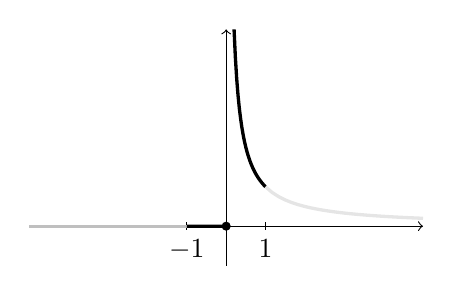
\begin{tikzpicture}[scale = 0.5]
		% axes
		\draw[->] (-5,  0) -- (5, 0);
		\draw[->] ( 0, -1) -- (0, 5);
		\draw (-1, 0.1) -- (-1, -0.1) node[below]{$-1$};
		\draw (1, 0.1) -- (1, -0.1) node[below]{$1$};
		% the line part
		\draw[very thick, gray!50] (-5, 0) -- (-1, 0);
		\draw[very thick, fill] (-1, 0) -- (0,0) circle (0.07);
		% the curver part
		\draw[very thick, domain=0.2:1] plot (\x,{1/\x});
		\draw[very thick, domain=1:5, gray!20] plot (\x,{1/\x});
	\end{tikzpicture}
	\caption{A non-continuous function~$[-1, 1] \to ℝ$ with closed graph.}
	\label{non-continuous function with closed graph}
\end{figure}

This begs the following question:
\begin{quote}
	Let~$Y$ be a topological space such that for every other topological space~$X$, every map~$f \colon X \to Y$ with closed graph is continuous.
	Then must~$Y$ be compact?
\end{quote}
The author doesn’t know the answer to this question.

\subsection{Exercise~2.21}

We will use the following generalization of Theorem~2.18.

\begin{proposition}
	\label{separating compact subspaces of hausdorff spaces}
	Let~$X$ be a Hausdorff space and let~$K$ and~$L$ be two disjoint compact subspaces of~$X$.
	There exist disjoint open subsets~$U$ and~$V$ of~$X$ with~$K ⊆ U$ and~$L ⊆ V$.
\end{proposition}

\begin{proof}
	We know from Theorem~2.18 that there exists for every point~$x$ in~$L$ disjoint open subsets~$U_x$ and~$V_x$ of~$X$ with~$K ⊆ U_x$ and~$x ∈ V_x$.
	The resulting open cover~$\{ V_x \suchthat x ∈ L \}$ of~$L$ admits a finite subcover, indexed by points~$x_1, \dotsc, x_n$.
	We set~$U ≔ ⋂_{i = 1}^n U_{x_i}$ and~$V ≔ ⋃_{i = 1}^n V_{x_i}$.
\end{proof}

Let~$x$ and~$y$ be two distinct points in~$Y$.
The fibres~$f^{-1} x$ and~$f^{-1} y$ are disjoint compact subspaces of~$X$.
It follows from the above \lcnamecref{separating compact subspaces of hausdorff spaces} that there exist disjoint open subsets~$U'$ and~$V'$ of~$X$ with~$f^{-1} x ⊆ U'$ and~$f^{-1} y ⊆ V'$.

We can now proceed in two ways.

\subsubsection{First Argumentation}

We note that the continuous surjection~$f$ is a quotient map because it is closed, see Exercise~1.14.
So for every saturated open subset of~$X$, its image in~$Y$ is again open.
We will therefore replace~$U'$ and~$V'$ by smaller open subsets~$U$ and~$V$ that are saturated with respect to~$f$, but still separate the two fibres~$f^{-1} x$ and~$f^{-1} y$.

The complement~$C' ≔ X ∖ U'$ is closed in~$X$.
Its image~$f C'$ is closed in~$Y$ because~$f$ is closed, and the preimage~$C ≔ f^{-1} f C'$ is again closed in~$X$ because~$f$ is continuous.
The complement~$U ≔ X ∖ C$ is therefore open in~$X$.
We have~$C' ⊆ C$ and thus~$U ⊆ U'$.
The fibre~$f^{-1} x$ is disjoint to~$C'$, so~$x$ is not contained in~$f C'$, and therefore~$C$ is again disjoint to~$f^{-1} x$.
Consequently, the fibre~$f^{-1} x$ is contained in~$U$.
Since~$C$ is saturated with respect to~$f$, so is its complement~$U$.

We can construct in the same way an open subset~$V$ of~$X$ such that the fibre~$f^{-1} y$ is contained in~$V$, we have~$V ⊆ V'$, and the set~$V$ is saturated with respect to~$f$.

The image sets~$f U$ and~$f V$ are open in~$Y$ because~$f$ is a quotient map and~$U$ and~$V$ are open and saturated with respect to~$f$.
The sets~$f U$ and~$f V$ are again disjoint because~$U$ and~$V$ are disjoint and saturated with respect to~$f$.
Finally,~$x$ lies in~$f U$ while~$y$ lies in~$f V$.

We have thus shown that the points of~$Y$ can be separated by disjoint open sets.
In other words,~$Y$ is again a Hausdorff space.

\subsubsection{Second Argumentation}

We consider the complements~$C' ≔ X ∖ U'$ and~$D' ≔ X ∖ V'$.
These are two closed subsets of~$X$ with~$X = C' ∪ D'$ because~$U'$ and~$V'$ are disjoint.
The image sets~$C ≔ f C'$ and~$D ≔ f D'$ are closed in~$Y$ because the map~$f$ is closed, and they satisfy
\[
	C ∪ D = f C' ∪ f D' = f (C' ∪ D') = f X = Y \,.
\]

The complements~$U ≔ Y ∖ C$ and~$V ≔ Y ∖ D$ are therefore disjoint open subsets of~$Y$.
The fibre~$f^{-1} x$ lies in~$U'$, is therefore disjoint to~$C'$, whence~$x$ does not lie in~$C$, so that~$x$ lies in~$U$.
We find in the same way that~$y$ lies in~$V$.

